%This is my super simple Real Analysis Homework template

\documentclass{article}

%% Language and font encodings
\usepackage[T1,T8K,T8M]{fontenc}
\usepackage[utf8]{inputenc}
\usepackage[english,georgian]{babel}

\usepackage{amsmath}
\usepackage{graphicx}
\usepackage[colorinlistoftodos]{todonotes}
\usepackage[colorlinks=true, allcolors=blue]{hyperref}
\usepackage{float}
\usepackage{enumerate}
\usepackage{subfig}
\usepackage{gensymb}

%\title{დავალება 01}
%\author{Your Name}
%\date\today
%This information doesn't actually show up on your document unless you use the maketitle command below

\begin{document}

\subsection{ამოცანა 1}
%წყარო?
განსაზღვრე წნევა $S$ კვეთისა და $m$ მასის მცურავი ცილინდრის ქვედა ზედაპირზე, თუ ატმოსფერული წნევაა $P_0$
		
\subsection{ამოცანა 2}
%წყარო უცნობი
$m$ მასის თხელკედლიანი ჭიქა ვერტიკალურად დაცურავს $\rho_1$ და $\rho_2$ სიმკვრივის ორი სითხის გამყოფ საზღვარზე. განსაზღვრეთ ქვედა სითხეში ჭიქის ჩაძირვის სიღრმე, თუ ჭიქის ფსკერის სისქეა $h$, განიკვეთის ფართობი - $S$, ხოლო ჭიქა შევსებულია $\rho_1$ სიმკვრივის სითხით.
\begin{figure}[h]
  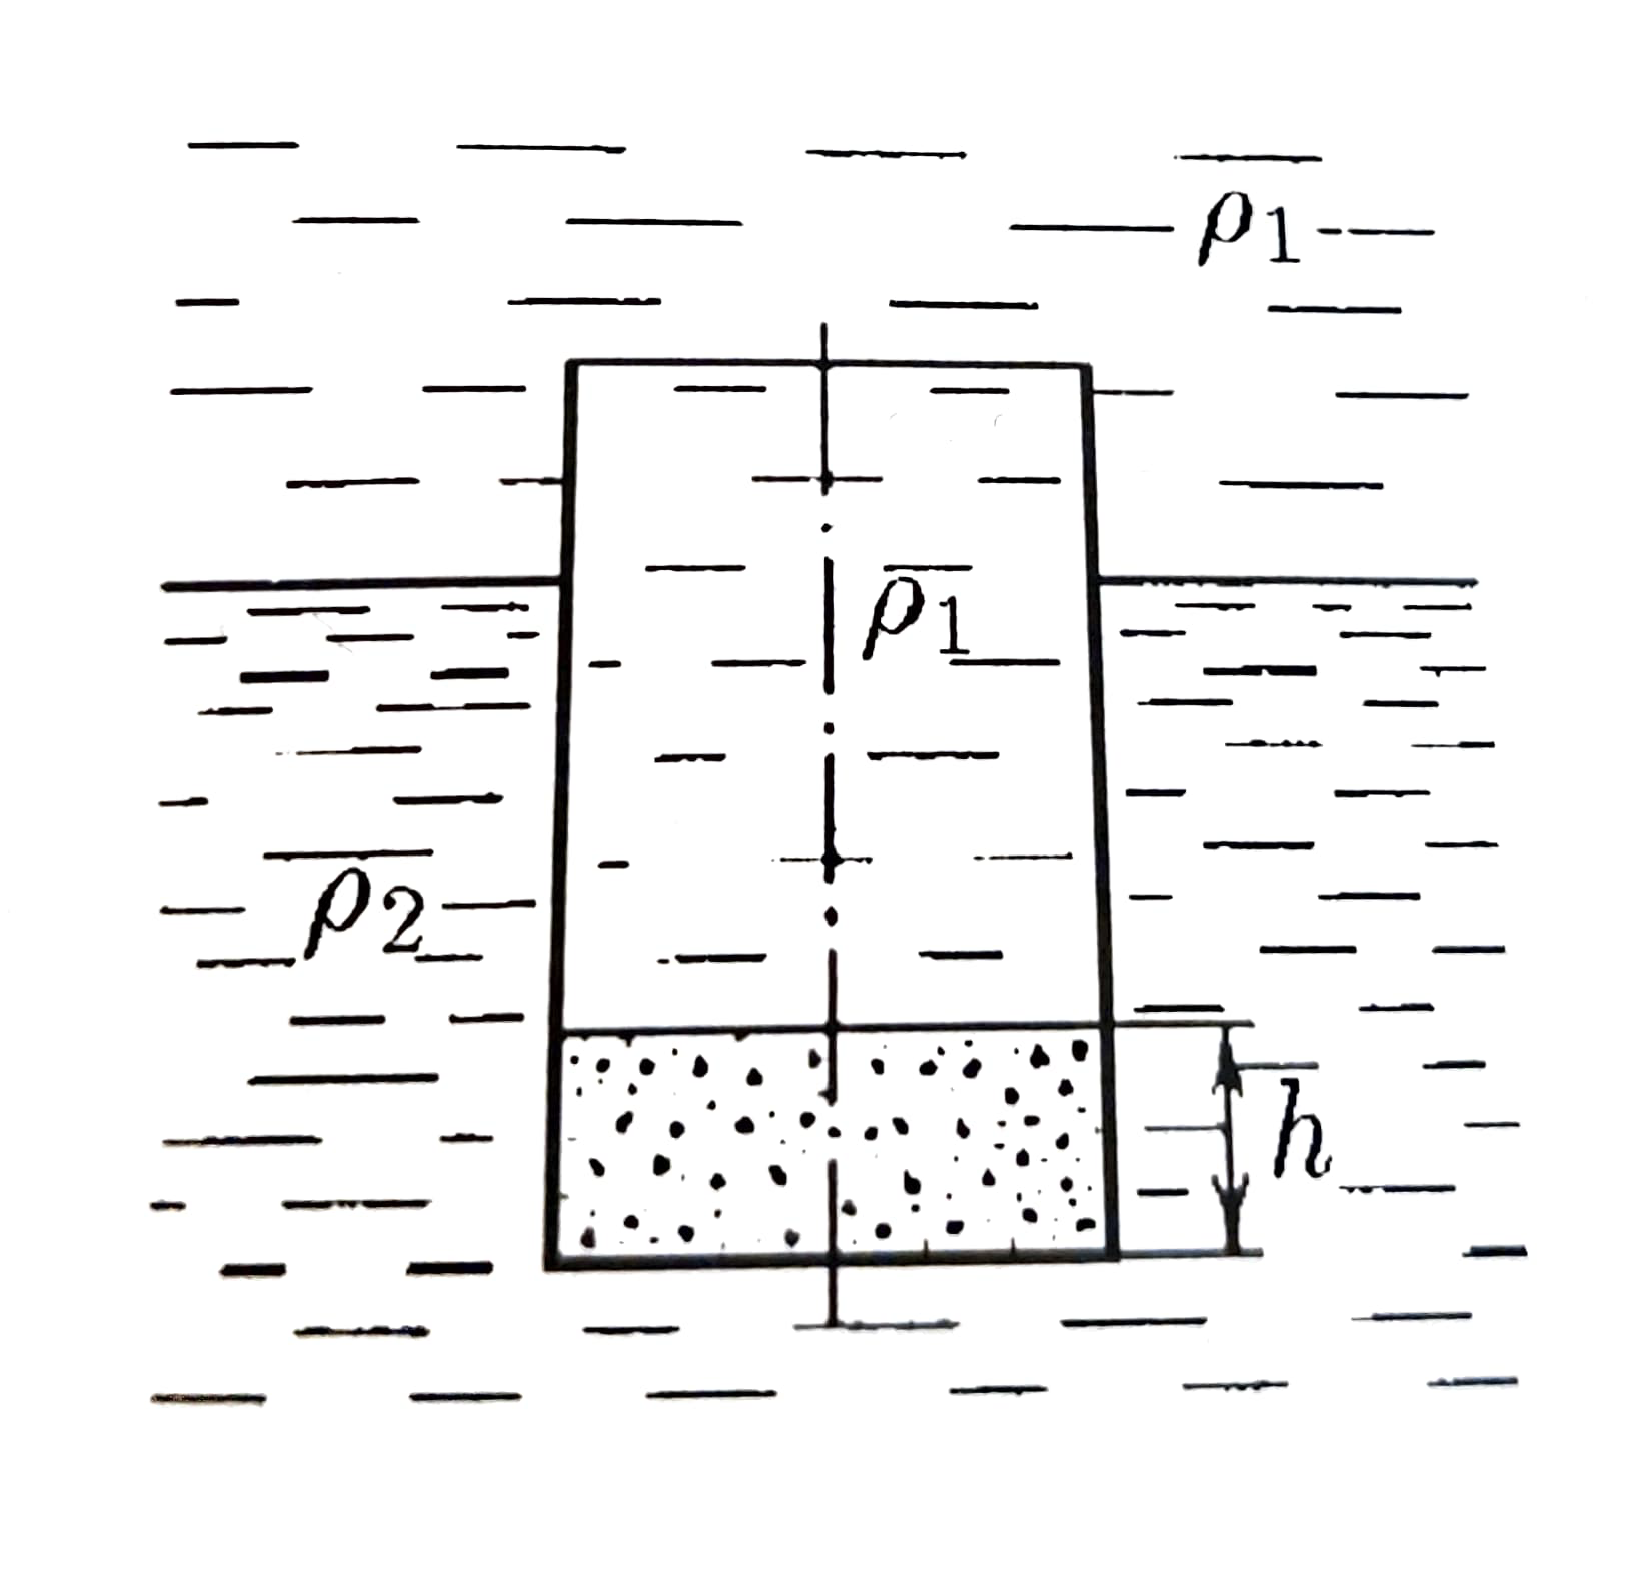
\includegraphics[width = .5\textwidth]{figures/figure_02}
  \caption{A boat.}
  \label{fig:boat1}
\end{figure}

\subsection{ამოცანა 3}
ორი თითოეული $10 სმ^{3}$ მოცულობის ბურთულა გადაბმულია ძაფით. განსაზღვრე ძაფის დაჭიმულობის ძალა, თუ ზედა ბურთულა წყალში ნახევრად ჩაძირული ტივტივებს. ქვედა ბურთულა ზედაზე სამჯერ მეტია. 

\subsection{ამოცანა 4}
ა) რა ნივთიერებისაგან უნდა იყოს დამზადებული გირი, რომ ზუსტი აწონვებისას არ დაგვჭირდეს ჰაერით გამოწვეული მასის "დაკარგვის" შესწორება. \\
ბ) წყლიან ჭურჭელში ვერტიკალურ მდგომარეობაში დაცურავს მართკუთხა ძელაკი, როგორ შეიცვლება წყლის დონე ჭურჭელში თუ ძელაკი გადავა ჰორიზონტალურ მდგომარეობაში.
\end{document}